\documentclass{standalone}
\usepackage{tikz}
\usetikzlibrary{patterns, positioning}


\begin{document}
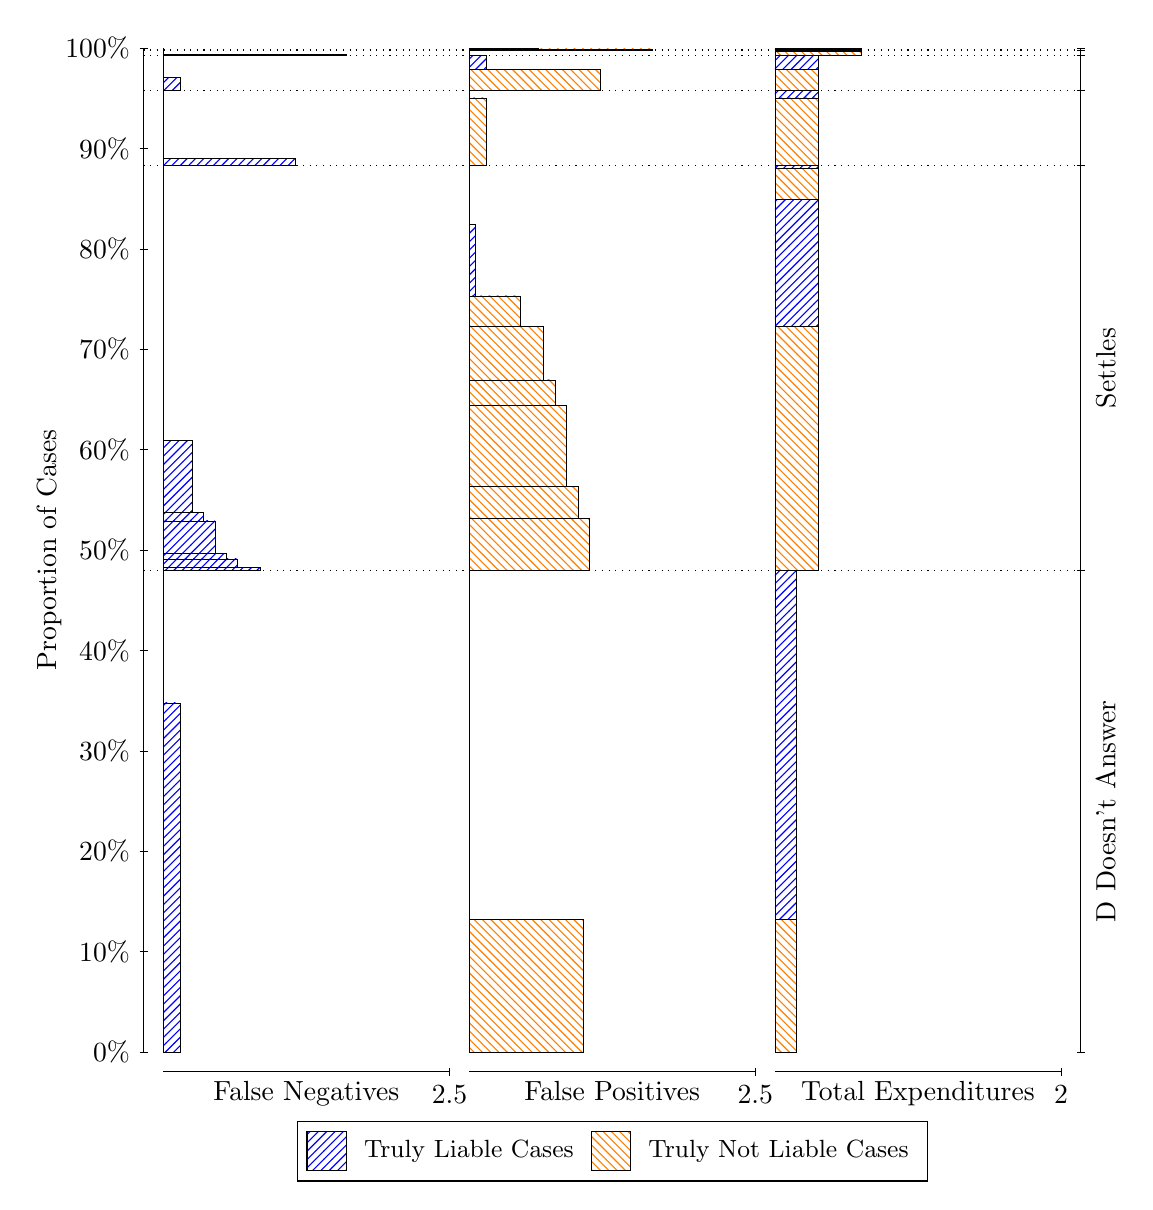
\begin{tikzpicture}
\draw[black, very thin] (1.5,1.75) -- (1.5,14.5);
\node[rotate=90, text=black, anchor=center] at (0.3, 8.125) {Proportion of Cases};
\draw[black, very thin] (1.45,1.75) -- (1.55,1.75);
\node[text=black, anchor=east] at (1.45, 1.75) {0\%};
\draw[black, very thin] (1.45,3.025) -- (1.55,3.025);
\node[text=black, anchor=east] at (1.45, 3.025) {10\%};
\draw[black, very thin] (1.45,4.3) -- (1.55,4.3);
\node[text=black, anchor=east] at (1.45, 4.3) {20\%};
\draw[black, very thin] (1.45,5.575) -- (1.55,5.575);
\node[text=black, anchor=east] at (1.45, 5.575) {30\%};
\draw[black, very thin] (1.45,6.85) -- (1.55,6.85);
\node[text=black, anchor=east] at (1.45, 6.85) {40\%};
\draw[black, very thin] (1.45,8.125) -- (1.55,8.125);
\node[text=black, anchor=east] at (1.45, 8.125) {50\%};
\draw[black, very thin] (1.45,9.4) -- (1.55,9.4);
\node[text=black, anchor=east] at (1.45, 9.4) {60\%};
\draw[black, very thin] (1.45,10.675) -- (1.55,10.675);
\node[text=black, anchor=east] at (1.45, 10.675) {70\%};
\draw[black, very thin] (1.45,11.95) -- (1.55,11.95);
\node[text=black, anchor=east] at (1.45, 11.95) {80\%};
\draw[black, very thin] (1.45,13.225) -- (1.55,13.225);
\node[text=black, anchor=east] at (1.45, 13.225) {90\%};
\draw[black, very thin] (1.45,14.5) -- (1.55,14.5);
\node[text=black, anchor=east] at (1.45, 14.5) {100\%};

\draw[black, very thin] (13.4,1.75) -- (13.4,14.5);
\draw[black, very thin] (13.35,1.75) -- (13.45,1.75);
\node[anchor=west] at (13.35, 1.75) {};
\draw[black, very thin] (13.35,7.866) -- (13.45,7.866);
\node[anchor=west] at (13.35, 7.866) {};
\draw[black, very thin] (13.35,13.005) -- (13.45,13.005);
\node[anchor=west] at (13.35, 13.005) {};
\draw[black, very thin] (13.35,13.96) -- (13.45,13.96);
\node[anchor=west] at (13.35, 13.96) {};
\draw[black, very thin] (13.35,14.402) -- (13.45,14.402);
\node[anchor=west] at (13.35, 14.402) {};
\draw[black, very thin] (13.35,14.475) -- (13.45,14.475);
\node[anchor=west] at (13.35, 14.475) {};
\draw[black, very thin] (13.35,14.5) -- (13.45,14.5);
\node[anchor=west] at (13.35, 14.5) {};

\draw[black, very thin, pattern color=blue, pattern=north east lines] (1.75,1.75) rectangle (1.968,6.182);
\draw[black, very thin, pattern color=orange, pattern=north west lines] (1.75,6.182) rectangle (1.75,7.866);
\draw[black, very thin, pattern color=blue, pattern=north east lines] (1.75,7.866) rectangle (2.9853,7.9028);
\draw[black, very thin, pattern color=blue, pattern=north east lines] (1.75,7.9028) rectangle (2.6947,8.0114);
\draw[black, very thin, pattern color=blue, pattern=north east lines] (1.75,8.0114) rectangle (2.5493,8.0835);
\draw[black, very thin, pattern color=blue, pattern=north east lines] (1.75,8.0835) rectangle (2.404,8.4952);
\draw[black, very thin, pattern color=blue, pattern=north east lines] (1.75,8.4952) rectangle (2.2587,8.6073);
\draw[black, very thin, pattern color=blue, pattern=north east lines] (1.75,8.6073) rectangle (2.1133,9.52);
\draw[black, very thin, pattern color=orange, pattern=north west lines] (1.75,9.52) rectangle (1.75,13.005);
\draw[black, very thin, pattern color=blue, pattern=north east lines] (1.75,13.005) rectangle (3.4213,13.097);
\draw[black, very thin, pattern color=orange, pattern=north west lines] (1.75,13.097) rectangle (1.75,13.96);
\draw[black, very thin, pattern color=blue, pattern=north east lines] (1.75,13.96) rectangle (1.968,14.131);
\draw[black, very thin, pattern color=orange, pattern=north west lines] (1.75,14.131) rectangle (1.75,14.402);
\draw[black, very thin, pattern color=blue, pattern=north east lines] (1.75,14.402) rectangle (4.0753,14.416);
\draw[black, very thin, pattern color=orange, pattern=north west lines] (1.75,14.416) rectangle (1.75,14.475);
\draw[black, very thin, pattern color=orange, pattern=north west lines] (1.75,14.475) rectangle (1.75,14.489);
\draw[black, very thin, pattern color=blue, pattern=north east lines] (1.75,14.489) rectangle (1.75,14.5);
\draw[black, very thin, pattern color=orange, pattern=north west lines] (5.6333,1.75) rectangle (7.0867,3.434);
\draw[black, very thin, pattern color=blue, pattern=north east lines] (5.6333,3.434) rectangle (5.6333,7.866);
\draw[black, very thin, pattern color=orange, pattern=north west lines] (5.6333,7.866) rectangle (7.1593,8.5219);
\draw[black, very thin, pattern color=orange, pattern=north west lines] (5.6333,8.5219) rectangle (7.014,8.9361);
\draw[black, very thin, pattern color=orange, pattern=north west lines] (5.6333,8.9361) rectangle (6.8687,9.9611);
\draw[black, very thin, pattern color=orange, pattern=north west lines] (5.6333,9.9611) rectangle (6.7233,10.286);
\draw[black, very thin, pattern color=orange, pattern=north west lines] (5.6333,10.286) rectangle (6.578,10.964);
\draw[black, very thin, pattern color=orange, pattern=north west lines] (5.6333,10.964) rectangle (6.2873,11.351);
\draw[black, very thin, pattern color=blue, pattern=north east lines] (5.6333,11.351) rectangle (5.706,12.263);
\draw[black, very thin, pattern color=blue, pattern=north east lines] (5.6333,12.263) rectangle (5.6333,13.005);
\draw[black, very thin, pattern color=orange, pattern=north west lines] (5.6333,13.005) rectangle (5.8513,13.867);
\draw[black, very thin, pattern color=blue, pattern=north east lines] (5.6333,13.867) rectangle (5.6333,13.96);
\draw[black, very thin, pattern color=orange, pattern=north west lines] (5.6333,13.96) rectangle (7.3047,14.231);
\draw[black, very thin, pattern color=blue, pattern=north east lines] (5.6333,14.231) rectangle (5.8513,14.402);
\draw[black, very thin, pattern color=orange, pattern=north west lines] (5.6333,14.402) rectangle (5.6333,14.461);
\draw[black, very thin, pattern color=blue, pattern=north east lines] (5.6333,14.461) rectangle (5.6333,14.475);
\draw[black, very thin, pattern color=orange, pattern=north west lines] (5.6333,14.475) rectangle (7.9587,14.489);
\draw[black, very thin, pattern color=blue, pattern=north east lines] (5.6333,14.489) rectangle (6.5053,14.5);
\draw[black, very thin, pattern color=orange, pattern=north west lines] (9.5167,1.75) rectangle (9.7892,3.434);
\draw[black, very thin, pattern color=blue, pattern=north east lines] (9.5167,3.434) rectangle (9.7892,7.866);
\draw[black, very thin, pattern color=orange, pattern=north west lines] (9.5167,7.866) rectangle (10.062,10.964);
\draw[black, very thin, pattern color=blue, pattern=north east lines] (9.5167,10.964) rectangle (10.062,12.581);
\draw[black, very thin, pattern color=orange, pattern=north west lines] (9.5167,12.581) rectangle (10.062,12.968);
\draw[black, very thin, pattern color=blue, pattern=north east lines] (9.5167,12.968) rectangle (10.062,13.005);
\draw[black, very thin, pattern color=orange, pattern=north west lines] (9.5167,13.005) rectangle (10.062,13.867);
\draw[black, very thin, pattern color=blue, pattern=north east lines] (9.5167,13.867) rectangle (10.062,13.96);
\draw[black, very thin, pattern color=orange, pattern=north west lines] (9.5167,13.96) rectangle (10.062,14.231);
\draw[black, very thin, pattern color=blue, pattern=north east lines] (9.5167,14.231) rectangle (10.062,14.402);
\draw[black, very thin, pattern color=orange, pattern=north west lines] (9.5167,14.402) rectangle (10.607,14.461);
\draw[black, very thin, pattern color=blue, pattern=north east lines] (9.5167,14.461) rectangle (10.607,14.475);
\draw[black, very thin, pattern color=orange, pattern=north west lines] (9.5167,14.475) rectangle (10.607,14.489);
\draw[black, very thin, pattern color=blue, pattern=north east lines] (9.5167,14.489) rectangle (10.607,14.5);
\draw[black, dotted] (1.5,7.866) -- (13.4,7.866);
\draw[black, dotted] (1.5,13.005) -- (13.4,13.005);
\draw[black, dotted] (1.5,13.96) -- (13.4,13.96);
\draw[black, dotted] (1.5,14.402) -- (13.4,14.402);
\draw[black, dotted] (1.5,14.475) -- (13.4,14.475);
\draw[black, very thin] (1.75,1.5) -- (5.3833,1.5);
\node[text=black, anchor=north] at (3.5667, 1.5) {False Negatives};
\draw[black, very thin] (5.3833,1.45) -- (5.3833,1.55);
\node[text=black, anchor=north] at (5.3833, 1.45) {2.5};

\draw[black, very thin] (5.6333,1.5) -- (9.2667,1.5);
\node[text=black, anchor=north] at (7.45, 1.5) {False Positives};
\draw[black, very thin] (9.2667,1.45) -- (9.2667,1.55);
\node[text=black, anchor=north] at (9.2667, 1.45) {2.5};

\draw[black, very thin] (9.5167,1.5) -- (13.15,1.5);
\node[text=black, anchor=north] at (11.333, 1.5) {Total Expenditures};
\draw[black, very thin] (13.15,1.45) -- (13.15,1.55);
\node[text=black, anchor=north] at (13.15, 1.45) {2};

\node[text=black, centered, rotate=90] at (13.72, 4.808) {D Doesn't Answer};
\node[text=black, centered, rotate=90] at (13.72, 10.435) {Settles};





\draw (7.449999999999999,1.5) node[draw=none] (baseCoordinate) {};
\begin{scope}[align=center]
        \matrix[scale=0.5, draw=black, below=0.5cm of baseCoordinate, nodes={draw}, column sep=0.1cm]{
            \node[rectangle, draw, minimum width=0.5cm, minimum height=0.5cm, pattern color=blue, pattern=north east lines] {}; &
            \node[draw=none, font=\small, text=black] (B) {Truly Liable Cases}; &
            \node[rectangle, draw, minimum width=0.5cm, minimum height=0.5cm, pattern color=orange, pattern=north west lines] {}; &
            \node[draw=none, font=\small, text=black] (B) {Truly Not Liable Cases}; \\
            };
\end{scope}

\end{tikzpicture}
\end{document}